\documentclass{article}
\usepackage{lmodern} % Latin Modern Font
\usepackage[T1]{fontenc}
\usepackage{amsfonts} % \mathbb
\usepackage[margin=0.5in]{geometry}
\usepackage[utf8]{inputenc}
\usepackage{graphicx}
% \graphicspath{{images/}}
\usepackage[backend=biber]{biblatex}
\usepackage{amsmath}
\usepackage[makeroom]{cancel}
% \usepackage{auto-pst-pdf}

% \usepackage{hyperref}
% \usepackage{hypcap}
% \DeclareMathOperator{\sign}{sign}
% \hypersetup{
%   colorlinks=true, 
%   allcolors=black,
%   pdfauthor={Carlos Henrique Tarjano Santos},
%   pdftitle={Robust Digital Envelope Estimation Via Geometric Properties of an Arbitrary Real Signal}
% }

\bibliography{bibli}

\usepackage{authblk}
\title{Title}
\author[1]{Carlos Henrique Tarjano Santos}
\author[2]{Valdecy Pereira}
\affil[1]{(corresponding author, carlostarjano@id.uff.br) Department of Production Engineering, Universidade Federal Fluminense, Rua Passo da Pátria, 156, Campus Praia Vermelha, Bloco D - sala 309, São Domingos, Niterói, RJ, Brasil, CEP: 24.210-240}
\affil[2]{Department of Production Engineering, Universidade Federal Fluminense, Rua Passo da Pátria, 156, Campus Praia Vermelha, Bloco D - sala 309, São Domingos, Niterói, RJ, Brasil, CEP: 24.210-240}



\begin{document}

\maketitle

\begin{abstract} % ≅ 250 words  
% Clear and simple miniature version of the paper
% Self-contained
% Past tense for the current study
% Present tense to refer to stablished facts

% Background (What is already known about the subject)

% Motivation (Why do we care about the problem and the results?) 

% Problem | Objectives (What problem is the paper trying to solve?) (Scope)

% Methods | Procedure | Approach (What did you actually do to get your results?)

% Results | Findings | Product (what did you learn | invent | create?)

% Conclusions | Implications (What are the larger implications of your findings)

\end{abstract}

{\bf Keywords:} 


\section{Introduction} % ≅ 500 words
% ≅ 10\% of the text
% broad to specific
% show that the research question is clear, concise, and worthy of study.
% allow the reader to understand the rest of the paper without referring to previous publications on the topic
% What did you do?
% conclusions

% Opener sentence (Question | Assertion | Intriguing Revelations)

% Literature review | Brief Context of Prior Research
  % put your research in the context of other research
  % Nature and scope of the problem investigated
  % give them a framework for understanding it
  % What is the problem to be solved?
  % Are there any existing solutions?
  % Which is the best?
  % What is its main limitation?
  % What do you hope to achieve?

% Restate Your Question as Something Not Known or Fully Understood by Prior Research
  % identify the gap in the literature
  % use but, however, etc…

% State the Significance of Your Question
  % make readers understand why they should read your report

% State Your Claim | Objective | Hypothesis
  % should clearly relate to the information gap
  
% brief outlook on the structure of the paper

\section{Methodology} % ≅ 1000 words
  % How did you do it?
  % Justify choices
  % Describe the work so as people can reproduce it

% Overview of methods

% Restate the purpose of the work

% Essential background information

% Relate to other studies

% Indicate where problems occurred



\section{Results} % ≅ 3000 words
  % What did you find?
  % Use figures, tables, etc.
  % Clearly and simply stated.

% Revisit purpose and methods

% Overview of results

% Key results in details

% Comparison with results in other works

% Comparison with predictions

% Problems with results

% Possible implications

\section{Discussion} % ≅ 2000 words

% Put results into a broader context.

% specific to broad

% What does it all mean?

% an interpretation of how each of the experiments supported your central hypothesis

% add in supporting findings from the literature

% what principles have been established or reinforced

\section{Conclusion} % ≅ 250 words
  % leave readers with a clear idea of your claim
  % make readers understand its importance
  % suggest further research
  % how the work advances the field?
  % significance and implications of the results
  % implications for broader application
  % research opportunities

% Restate Your Claim

% Point Out: New Significance | Practical Application | New Research


% \begin{figure}[ht!]
%   \centering
%      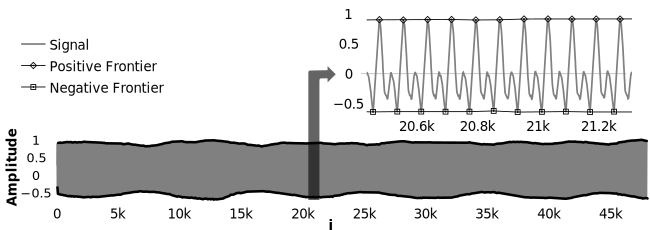
\includegraphics{images/01signalenvelope.pdf}
%   \caption{A discrete wave of the singing voice of an alto singer. The black lines are the frontiers; in the detail view, it can be seen that each region between two diamonds comprises a pseudo-cycle, as defined by the points belonging to the upper frontier. Similarly, two adjacent squares delimitate a pseudo-cycle, from the standpoint of the lower frontier.}
%   \label{fig:signalenvelope}
% \end{figure}



\printbibliography % 20 ⇔ 60 itens

\end{document}
